\documentclass[compress]{beamer}

% Inclusion des packages
%================== ENCODAGE & LANGUE ==================
\usepackage[utf8]{inputenc}
\usepackage[T1]{fontenc}
%\usepackage[french]{babel} % Optionnel

%================== MATHS & SYMBOLES ===================
\usepackage{amsmath, amssymb, amsfonts}
\usepackage{yhmath, mathdots, cancel}
\usepackage{siunitx}
\usepackage{gensymb}
\usepackage{textcomp}
\usepackage{pifont}
\usepackage{xspace}


%================== TABLEAUX ============================
\usepackage{array, tabularx, multirow, booktabs}

%================== COULEURS & GRAPHISMES ===============
\usepackage{color}
\usepackage{tikz}
\usetikzlibrary{
  shapes.geometric,
  backgrounds,
  fadings,
  patterns,
  shadows.blur,
  shapes,
  positioning,
  decorations.pathreplacing,
  matrix
}
\usepackage{tikz-3dplot}
\usepackage{asymptote}
\usepackage{xcolor}

%================== MISE EN PAGE ========================
\usepackage{changepage}
\usepackage{calc}
\usepackage{caption}
\usepackage{xspace}
\usepackage{ragged2e}
\usepackage{amsmath, amsfonts, mathtools, amsthm, amssymb}
\usepackage{adjustbox}
\usepackage{caption}
\usepackage{beamerappendixnote}
\usepackage{bookmark}


%================== ALGORITHMIQUE =======================
\usepackage[ruled,vlined]{algorithm2e}
\SetAlgorithmName{Algorithme}{Algo}{Liste des algorithmes}
\SetFuncArgSty{textup}
\SetArgSty{textup}
\SetKwFor{ForEach}{pour tout}{faire}{}
\SetKwFor{For}{pour}{faire}{finpour}
\SetKwIF{Si}{SinonSi}{Sinon}{si}{alors}{sinon si}{sinon}{}
\SetKwInput{Input}{Entrée}
\SetKwInput{Output}{Sortie}
\SetKwProg{myproc}{Procédure}{:}{}
\SetKw{Return}{retourner}
\SetKwComment{tcc}{(*}{*)}
\SetKwFor{Tq}{tant que}{faire}{}
\SetKwRepeat{Repeter}{répéter}{jusqu’à}
\renewcommand{\thealgocf}{}
%================== AUTRES ==============================
\usepackage[clock]{ifsym}



% Définir les initiales pour affichage dans l'en-tête (à utiliser dans thème perso si besoin)
\newcommand{\initiales}{L.-H. Cuingnet}

% Commandes utilitaires
\newcommand{\lin}[1]{\texttt{#1}} % Évite minted si pas nécessaire
\newcommand{\flch}{\item[$\rightarrow$]}
\newcommand{\dc}{{\usebeamercolor[fg]{structure}$\hookrightarrow$}}
\newcommand{\ok}{\textcolor{green}{\checkmark}}
\newcommand{\point}{{\usebeamercolor[fg]{structure}$\bullet\enskip$}}
\newcommand{\Point}{\point}
\newcommand{\couleur}[1]{{\usebeamercolor[fg]{structure}#1}}
\newcommand{\important}[1]{\couleur{\textbf{#1}}}
\newcommand{\remarque}[1]{\textit{\textrm{#1}}}

% Paramètres Beamer et thème (à personnaliser dans ce fichier)
\usetheme{CambridgeUS}
\usecolortheme{seahorse}


%--------marges
\setbeamersize{text margin left= 0.7cm}
\setbeamersize{text margin right= 0.7cm}

%--------tête et pieds
\setbeamertemplate{navigation symbols}{}
\setbeamertemplate{footline}[frame number]
\setbeamertemplate{headline}{
  %la premiere ligne
  	\begin{beamercolorbox}[ht=0.42cm, vmode]{section in head/foot}
	\hspace{0.4cm} \insertshorttitle 
	\hspace*{0.1cm}- \initiales - {\insertshortdate}
	\vspace*{0.08cm} 
  	\end{beamercolorbox}
  %la deuxième ligne
	\begin{beamercolorbox}[ht=0.4cm, vmode]{subsection in head/foot}
	%titre de la section si elle est pas 0
		\ifnum\value{section}=0{} 
		\else{ \hspace{0.8cm} \thesection - \insertsectionhead }
		\fi
	%séparateur + titre de la sous-section si elle est pas 0
		\ifnum\value{subsection}=0{} 
		\else{ 
			\hspace*{0.1cm} \couleur{$\bullet$} \hspace*{0.1cm} 
			\thesection.\thesubsection \, \insertsubsectionhead
		}
		\fi
		\vspace*{0.12cm}
\end{beamercolorbox}
%\vspace*{-0.03cm} %pour pas qu'il y ait d'espace avec la ligne de frametitle
 }
%\setbeamertemplate{frametitleheigth}{4cm}
\setbeamertemplate{frametitle}{
	\vspace*{-0.04cm} 
	\begin{beamercolorbox}[ht=0.8cm,wd=\paperwidth, vmode]{frametitle}
		\hspace{0.3cm} \insertframetitle \vspace*{0.1cm}
	\end{beamercolorbox}
}

%commande pour ajuster l'alignement vertical des titres sans lettres descendantes
%\newcommand{\esp}{\\[0.1cm]} %--version qui marche sans le package minted
\newcommand{\esp}{\\[-0.5cm]} %--version qui marche avec le package minted


%--------couleurs
\setbeamercolor{structure}{fg=turquoiseFonce!70!black} 

\setbeamercolor{block title}{fg=turquoiseFonce!70!black,bg=vertdEau}
\setbeamercolor{block body}{bg=vertdEau!10!white}

\setbeamercolor{block title alerted}{bg=vertdEau!85!white,fg=turquoiseFonce!80!black}
\setbeamercolor{block body alerted}{bg=vertdEau!8!white}
%\setbeamercolor{alerted text}{fg=red}

\setbeamercolor{block title example}{bg=vertdEau,fg=turquoiseFonce}
\setbeamercolor{block body example}{bg=vertdEau!10!white}
\setbeamercolor{example text}{fg=blue!20!turquoise}

%-------- TOC
\setbeamertemplate{section in toc}[sections numbered]

%-----------------------------------------------
%Plan qui s'affiche au début de chaque section %|
\AtBeginSection[]{                             %|
\begin{frame}[plain]                           %|
\frametitle{Plan\\[0.1cm]}                     %|
\tableofcontents[                              %|
currentsection,                                %|
hideothersubsections,                          %|
subsubsectionstyle=hide]                       %|
\addtocounter{framenumber}{-1}                 %|
\end{frame}}                                   %|
%-----------------------------------------------




%-------- commande pour les ref sur les slides
\newcommand{\bandeauREF}[1]{
\noindent\makebox[\textwidth][l]{%
\hspace{-\dimexpr\oddsidemargin+1in}%
\colorbox{expli!20!white}{%
\parbox{\dimexpr\paperwidth-2\fboxsep}{
\footnotesize\textcolor{expli!80!black}{#1}
}}}}
% Commandes utilitaires
\tikzset{every picture/.style={line width=0.75pt}} %set default line width to 0.75pt        
\newcommand{\imageFrame}{
  \draw [line width=0.75] (261.98,12.03) -- (262.02,142.84) -- (150.52,236.47) -- (150.47,105.66) -- cycle ;
}
\newcommand{\lin}[1]{\texttt{#1}} % Évite minted si pas nécessaire
\newcommand{\flch}{\item[$\rightarrow$]}
\newcommand{\dc}{{\usebeamercolor[fg]{structure}$\hookrightarrow$}}
\newcommand{\ok}{\textcolor{green}{\checkmark}}
\newcommand{\point}{{\usebeamercolor[fg]{structure}$\bullet\enskip$}}
\newcommand{\Point}{\point}
\newcommand{\couleur}[1]{{\usebeamercolor[fg]{structure}#1}}
\newcommand{\important}[1]{\couleur{\textbf{#1}}}
\newcommand{\remarque}[1]{\textit{\textrm{#1}}}
\newcommand{\cmark}{\ding{51}\xspace} % check ✓
\newcommand{\xmark}{\ding{55}\xspace} % cross ✗

% Palette de couleurs personnalisée
%%%%%%%%%%%%%% couleurs locales
\newcommand{\cearly}{orange!50!oranger}
\newcommand{\ctardy}{orange!50!oranger!50!magenta!50!violet}
\newcommand{\cmilieu}{yellow!45!magenta}
\newcommand{\cfenetre}{yellow!45!magenta}
%\newcommand{\cfenetre}{orange!80!magenta!80!violet}
\newcommand{\caxe}{blue!60!black}

\definecolor{vert}{RGB}{194, 247, 50}
\definecolor{vertClair}{RGB}{80, 180, 33}
\definecolor{vertFonce}{RGB}{20, 148, 20} 


\definecolor{turquoiseFonce}{RGB}{0, 149, 182} 
\definecolor{turquoise}{RGB}{0, 204, 203}
%\definecolor{turquoise}{RGB}{53, 123, 153} 
\colorlet{monCyan}{turquoise!90!blue} 

\colorlet{vertdEau}{blue!50!green!30!white} 

\definecolor{prec}{RGB}{128, 0, 128} 
\definecolor{hyp}{RGB}{255, 0, 127} 


\definecolor{orange}{RGB}{250, 130, 1}
\definecolor{orange1}{RGB}{244, 142, 3}
\definecolor{orange2}{RGB}{255, 195, 0}
%\colorlet{orangé}{orange!55!yellow}
\colorlet{oranger}{orange!55!yellow}
\definecolor{jaune}{RGB}{255, 195, 0 }
\colorlet{ocre}{orange!90!green!80!white} 


\definecolor{briqueRouge}{RGB}{200, 48, 24}
\definecolor{brique}{RGB}{141, 48, 24}
\definecolor{brown}{RGB}{165, 137, 107}
\definecolor{chamois}{RGB}{200, 141, 75}

\colorlet{lavande}{vertdEau!50!blue}
\definecolor{lilas}{RGB}{154, 107, 165}
\colorlet{parme}{magenta} %violet!30!magenta
\definecolor{mauve}{RGB}{161, 132, 220}%{147, 112, 219}

\definecolor{prunelle}{RGB}{106,24, 141}
\definecolor{prune}{RGB}{121, 7, 123}
\definecolor{violet}{RGB}{153, 0, 139}
\definecolor{violette}{RGB}{128, 0, 128} 

\definecolor{rose}{RGB}{255, 0, 127} 
\definecolor{framboise}{RGB}{141, 24, 59}
\colorlet{grenat}{magenta!90!red!80!black}

\colorlet{expli}{gray}

\definecolor{hellseahorse}{RGB}{204, 204, 255}
\definecolor{seahorse}{RGB}{204,180, 255}
\definecolor{darkseahorse}{RGB}{83, 74, 196}

%================== DÉBUT DU DOCUMENT ===================
\begin{document}

\title[Reconstruction 3D]{Reconstruction d’objets convexes à partir de photographies}
\author{
  \large Présentation de \important{Lucie-Hélène Cuingnet}\\[0.2cm]
  \footnotesize Travail réalisé avec \couleur{Barnabé Baruchel}
}
\date[Mai 2025]{}

\begin{frame}[plain]
  \titlepage
  \addtocounter{framenumber}{-1}
\end{frame}

% Slides principales (actives selon les fichiers présents)
%%%%%%%%%%%%%%%%%%%%%%%%%%%%%%%%%%%%%%%%%%%%%%%%%
\section[Selection]{Selection}
%------------------------------------------------
\subsection{Points d'intérêts}
%++++++++++++++++++++++++++++++++++++++++++++++++
\begin{frame}{Points d'intérêts}
  \centering
  \note{
  La première étape consite à déterminer les points dont on doit déterminer les coordonnées 3D décrire notre objet. 
On appelera ces points les points d'intérêts, qu'on identifie à leur projection une image.
Par exemple ici sur un cube
}
  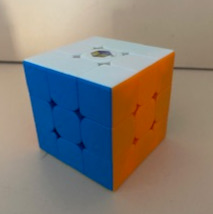
\includegraphics[width=0.6\textwidth]{capture/rub.jpg}
  \hyperlink{convex-appendix}{
    \beamerbutton{Contrainte de convexité}
  }
\end{frame}



\subsection{Algorithme}
%------------------------------------------------

\begin{frame}
  \label{algo-moravec}
\note{
L’algorithme de Moravec est un détecteur de coins assez simple basé sur la variation locale de l’intensité.
Pour chaque pixel, on mesure la variance de l’intensité dans plusieurs directions.
Si la plus petite variance dépasse un certain seuil, on considère qu’on est probablement sur un coin — une zone où l’image change dans toutes les directions.
}
  \hyperlink{moravec-appendix}{
    \beamerbutton{Exemple}
  }
	\small
\begin{algorithm}[H]
    \caption{\textsf{Séléction de points d'intérêts}}

    \only<1->{\KwIn{Image d’intensité \texttt{image}}}
    \only<2->{\KwOut{Matrice des coins détecté}}
    \only<3->{\BlankLine}
    \only<4->{\ForEach{pixel $(x, y)$ dans l’image}{%
        \only<5->{\Indp$scores \gets$ liste vide\;}}
        \only<6->{\ForEach{direction $(dx, dy)$ parmi : verticale, horizontale, diagonales}{%
            \only<7->{\Indp Calculer la variance locale autour de $(x, y)$ dans la direction $(dx, dy)$\;
            Ajouter la variance à $scores$\;}
        \Indm}
        }
        \only<8->{$score \gets \min(scores)$\;}
        \only<9->{\If{$score >$ \texttt{SEUIL}}{%
            \only<10->{\Indp Marquer $(x, y)$ comme coin\;}
        \Indm}
        }
    \Indm}
    \only<11->{\KwRet{Liste des points marqués}}
\end{algorithm}

\end{frame}

\subsection{Implémentation}

\begin{frame}{Fichier de sortie PBM}
  \note{"Une fois les coins détectés, on peut produire un fichier PBM, ici représenté à droite sous forme de matrice binaire.

Un ‘1’ correspond à un coin détecté. C’est ce fichier qui pourra être ensuite utilisé dans la suite du pipeline, notamment pour l’appariement."}
\begin{minipage}[c]{0.45\textwidth}
  \centering
  \begin{tikzpicture}
    \node[inner sep=0pt] (img) at (0,0) {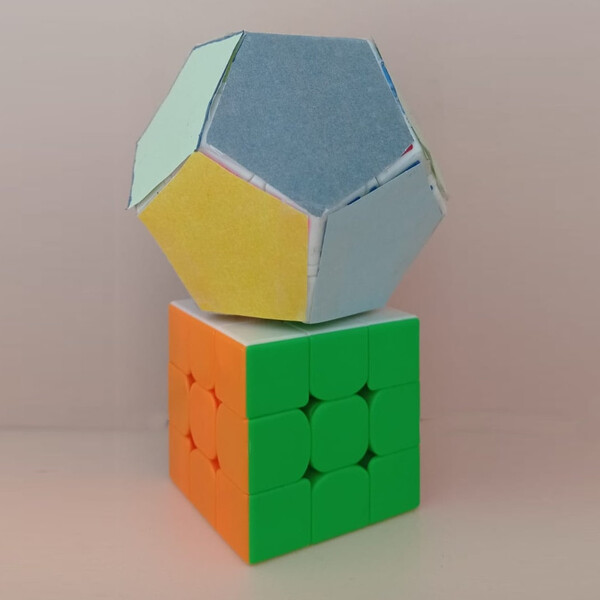
\includegraphics[width=0.9\textwidth]{capture/dodecf0.jpg}};
    \node at (3.5,0) {\Huge$\Rightarrow$};
  \end{tikzpicture}
\end{minipage}
\hfill
\begin{minipage}[c]{0.48\textwidth}
  \centering
  \renewcommand{\arraystretch}{1.2}
  \begin{tabular}{cccccc}
  0 & 0 & 0 & 0 & 0 & 0 \\
  0 & 1 & 1 & 0 & 0 & 0 \\
  0 & 1 & 0 & 1 & 1 & 0 \\
  0 & 0 & 1 & 0 & 0 & 0 \\
  0 & 0 & 1 & 1 & 0 & 0 \\
  0 & 0 & 0 & 1 & 1 & 0 \\
  0 & 1 & 1 & 0 & 0 & 1 \\
  0 & 1 & 0 & 1 & 1 & 0 \\
  0 & 0 & 1 & 0 & 0 & 0 \\
  0 & 0 & 1 & 1 & 0 & 0 \\
  \end{tabular}
\end{minipage}
\end{frame}

\begin{frame}{Influence des paramètres}
\note{"Voici quelques exemples de détection de coins selon différents paramètres.

On voit que si on change la taille de la fenêtre ou le seuil, le résultat est très différent.

Avec une fenêtre plus grande, on est plus tolérant au bruit mais on perd en précision.

Et avec un seuil plus faible, on détecte beaucoup plus de coins, parfois à tort.

Il est donc crucial d’ajuster ces paramètres selon les images qu’on traite."}
\begin{minipage}[c]{0.45\textwidth}
\raggedright
\small
\vspace*{\fill}

\textbf{Paramètres utilisés :}
\vspace{1em}

\begin{itemize}
  \setlength\itemsep{0.3em}
  \setlength\leftskip{1em}
  \only<1>{\item \textbf{THRESHOLD} = 2000 \\ \item \textbf{WINDOW} = 4}
  \only<2>{\item \textbf{THRESHOLD} = 2000 \\ \item \textbf{WINDOW} = 6}
  \only<3>{\item \textbf{THRESHOLD} = 4000 \\ \item \textbf{WINDOW} = 10}
  \only<4>{\item \textbf{THRESHOLD} = 500 \\ \item \textbf{WINDOW} = 2}
\end{itemize}

\vspace*{\fill}
\end{minipage}
\hfill
\begin{minipage}[c]{0.48\textwidth}
\centering
\begin{overlayarea}{0.9\linewidth}{4cm}

\only<1>{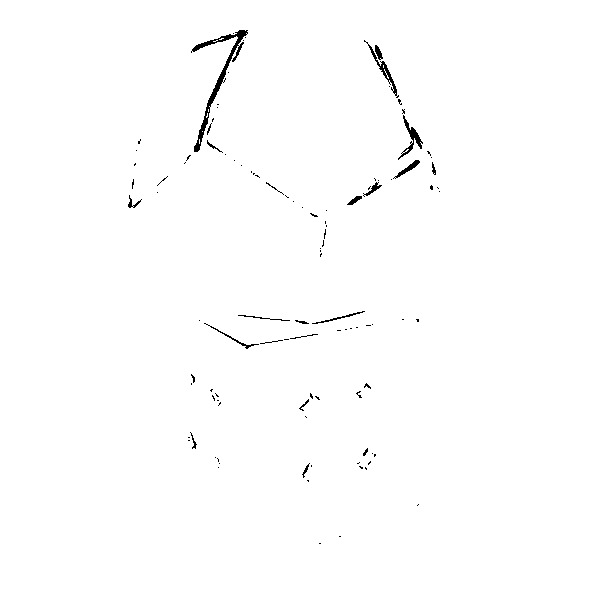
\includegraphics[width=0.9\textwidth]{capture/dodecf0-mv-2000-4-1.jpg}}
\only<2>{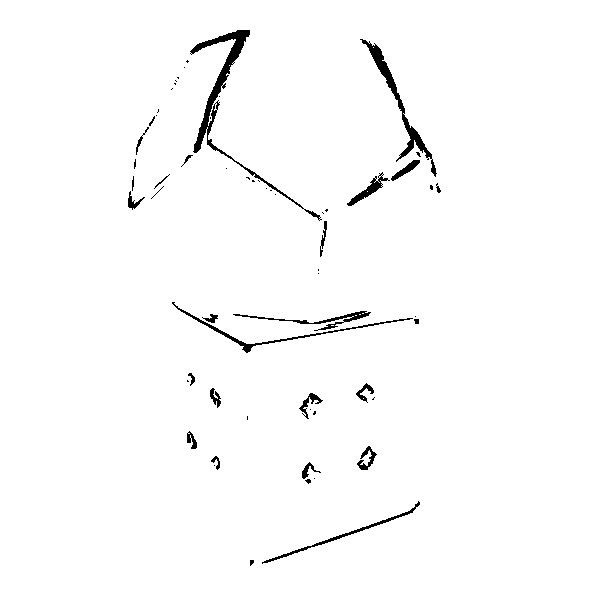
\includegraphics[width=0.9\textwidth]{capture/dodecf0-mv-2000-6-1.jpg}}
\only<3>{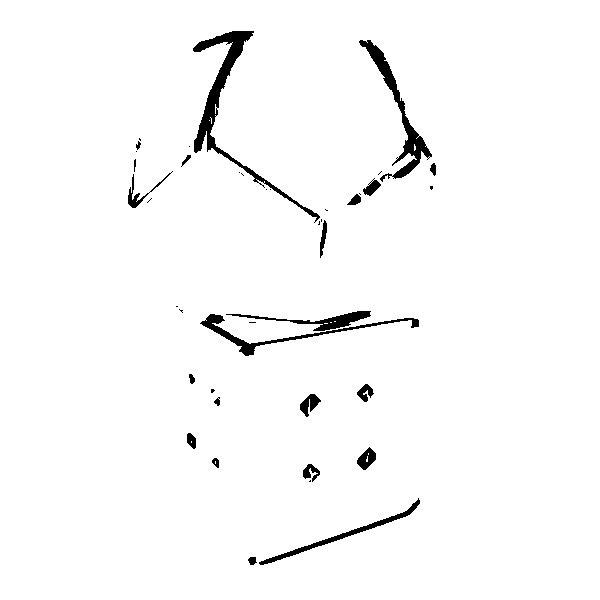
\includegraphics[width=0.9\textwidth]{capture/dodecf0-mv-4000-10-1.jpg}}
\only<4>{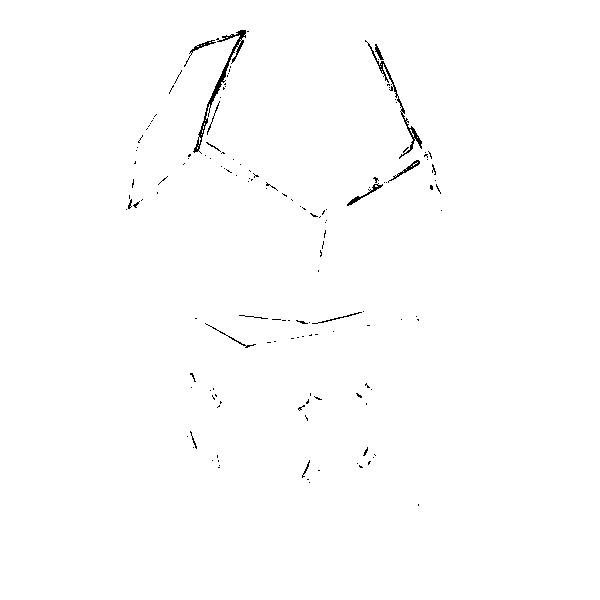
\includegraphics[width=0.9\textwidth]{capture/dodecf0-mv-500-2-1.jpg}}

\end{overlayarea}
\end{minipage}

\end{frame}

%%%%%%%%%%%%%%%%%%%%%%%%%%%%%%%%%%%%%%%%%%%%%%%%%
\section[Reconstruction]{Reconstruction}
%------------------------------------------------
\begin{frame}
\frametitle{Titre d'une slide avant la sous-section}
    Ici on n'a pas encore de titre de sous-section dans le bandeau du haut.
    \label{slides_hors_subsec}
\end{frame}

%++++++++++++++++++++++++++++++++++++++++++++++++
\subsection{Modélisation théorique}
%++++++++++++++++++++++++++++++++++++++++++++++++
\begin{frame}
\frametitle{Les différents repères}
  \begin{minipage}{0.58\textwidth}
        \scalebox{0.65}{


\tikzset{every picture/.style={line width=0.75pt}} %set default line width to 0.75pt        

\begin{tikzpicture}[x=0.75pt,y=0.75pt,yscale=-1,xscale=1]
%uncomment if require: \path (0,300); %set diagram left start at 0, and has height of 300

%Shape: Rectangle [id:dp9723727103024109] 
\draw  [line width=0.75]  (273.11,2.68) -- (273.16,155.68) -- (150.53,258.66) -- (150.47,105.66) -- cycle ;
%Shape: Circle [id:dp9239162914529644] 
\draw   (170.87,132.32) .. controls (172.23,131.96) and (173.33,132.77) .. (173.33,134.13) .. controls (173.33,135.49) and (172.23,136.89) .. (170.87,137.26) .. controls (169.5,137.62) and (168.4,136.81) .. (168.4,135.45) .. controls (168.4,134.09) and (169.5,132.69) .. (170.87,132.32) -- cycle ;
%Straight Lines [id:da4507743094695521] 
\draw  [dash pattern={on 0.84pt off 2.51pt}]  (211.82,130.67) -- (45,134.7) ;
%Shape: Circle [id:dp9335082203579057] 
\draw   (499.62,131.92) .. controls (500.98,131.55) and (502.08,132.36) .. (502.08,133.72) .. controls (502.08,135.09) and (500.98,136.49) .. (499.62,136.85) .. controls (498.25,137.22) and (497.15,136.41) .. (497.15,135.05) .. controls (497.15,133.68) and (498.25,132.28) .. (499.62,131.92) -- cycle ;
%Shape: Circle [id:dp5162114026007054] 
\draw  [color={rgb, 255:red, 241; green, 53; blue, 53 }  ,draw opacity=1 ] (512.82,105.92) .. controls (514.18,105.55) and (515.28,106.36) .. (515.28,107.72) .. controls (515.28,109.09) and (514.18,110.49) .. (512.82,110.85) .. controls (511.45,111.22) and (510.35,110.41) .. (510.35,109.05) .. controls (510.35,107.68) and (511.45,106.28) .. (512.82,105.92) -- cycle ;
%Shape: Circle [id:dp4319786220460511] 
\draw  [fill={rgb, 255:red, 0; green, 0; blue, 0 }  ,fill opacity=1 ] (321.12,132.42) .. controls (322.48,132.42) and (323.58,133.52) .. (323.58,134.88) .. controls (323.58,136.25) and (322.48,137.35) .. (321.12,137.35) .. controls (319.75,137.35) and (318.65,136.25) .. (318.65,134.88) .. controls (318.65,133.52) and (319.75,132.42) .. (321.12,132.42) -- cycle ;
%Straight Lines [id:da5164589906920809] 
\draw    (321.12,134.88) -- (321.97,70.75) ;
\draw [shift={(322,68.75)}, rotate = 90.77] [color={rgb, 255:red, 0; green, 0; blue, 0 }  ][line width=0.75]    (10.93,-3.29) .. controls (6.95,-1.4) and (3.31,-0.3) .. (0,0) .. controls (3.31,0.3) and (6.95,1.4) .. (10.93,3.29)   ;
%Straight Lines [id:da7854412907443913] 
\draw    (321.12,134.88) -- (253.5,134.75) ;
\draw [shift={(251.5,134.75)}, rotate = 0.11] [color={rgb, 255:red, 0; green, 0; blue, 0 }  ][line width=0.75]    (10.93,-3.29) .. controls (6.95,-1.4) and (3.31,-0.3) .. (0,0) .. controls (3.31,0.3) and (6.95,1.4) .. (10.93,3.29)   ;
%Straight Lines [id:da3058610918194634] 
\draw    (321.12,134.88) -- (272.48,176.16) ;
\draw [shift={(270.95,177.45)}, rotate = 319.68] [color={rgb, 255:red, 0; green, 0; blue, 0 }  ][line width=0.75]    (10.93,-3.29) .. controls (6.95,-1.4) and (3.31,-0.3) .. (0,0) .. controls (3.31,0.3) and (6.95,1.4) .. (10.93,3.29)   ;
%Straight Lines [id:da5453100201962917] 
\draw  [dash pattern={on 4.5pt off 4.5pt}]  (149.63,172.62) -- (150.47,105.66) ;
\draw [shift={(149.61,174.62)}, rotate = 270.72] [color={rgb, 255:red, 0; green, 0; blue, 0 }  ][line width=0.75]    (10.93,-3.29) .. controls (6.95,-1.4) and (3.31,-0.3) .. (0,0) .. controls (3.31,0.3) and (6.95,1.4) .. (10.93,3.29)   ;
%Straight Lines [id:da4691798453437107] 
\draw  [dash pattern={on 4.5pt off 4.5pt}]  (199.11,64.39) -- (150.47,105.66) ;
\draw [shift={(200.64,63.1)}, rotate = 139.68] [color={rgb, 255:red, 0; green, 0; blue, 0 }  ][line width=0.75]    (10.93,-3.29) .. controls (6.95,-1.4) and (3.31,-0.3) .. (0,0) .. controls (3.31,0.3) and (6.95,1.4) .. (10.93,3.29)   ;
%Straight Lines [id:da9224741393814412] 
\draw [color={rgb, 255:red, 241; green, 45; blue, 45 }  ,draw opacity=1 ]   (512.82,108.38) -- (192.48,152.97) ;
\draw [shift={(190.5,153.25)}, rotate = 352.08] [color={rgb, 255:red, 241; green, 45; blue, 45 }  ,draw opacity=1 ][line width=0.75]    (10.93,-3.29) .. controls (6.95,-1.4) and (3.31,-0.3) .. (0,0) .. controls (3.31,0.3) and (6.95,1.4) .. (10.93,3.29)   ;
%Shape: Circle [id:dp7585208638434278] 
\draw  [color={rgb, 255:red, 241; green, 53; blue, 53 }  ,draw opacity=1 ] (190.5,150.78) .. controls (191.86,150.42) and (192.97,151.23) .. (192.97,152.59) .. controls (192.97,153.95) and (191.86,155.35) .. (190.5,155.72) .. controls (189.14,156.08) and (188.03,155.27) .. (188.03,153.91) .. controls (188.03,152.55) and (189.14,151.15) .. (190.5,150.78) -- cycle ;
%Shape: Cube [id:dp7714367112041981] 
\draw   (499.62,131.92) -- (520.32,111.22) -- (568.62,111.22) -- (568.62,160.52) -- (547.92,181.22) -- (499.62,181.22) -- cycle ; \draw   (568.62,111.22) -- (547.92,131.92) -- (499.62,131.92) ; \draw   (547.92,131.92) -- (547.92,181.22) ;

% Text Node
\draw (517,97.9) node [anchor=north west][inner sep=0.75pt]  [font=\footnotesize,color={rgb, 255:red, 167; green, 17; blue, 17 }  ,opacity=1 ]  {$P$};
% Text Node
\draw (324,59.9) node [anchor=north west][inner sep=0.75pt]  [font=\footnotesize]  {$\vec{j}$};
% Text Node
\draw (280.5,178.9) node [anchor=north west][inner sep=0.75pt]  [font=\footnotesize]  {$\vec{i}$};
% Text Node
\draw (324.43,139.84) node [anchor=north west][inner sep=0.75pt]  [font=\footnotesize]  {$O$};
% Text Node
\draw (252,112.9) node [anchor=north west][inner sep=0.75pt]  [font=\footnotesize]  {$\vec{k}$};
% Text Node
\draw (158.65,118.28) node [anchor=north west][inner sep=0.75pt]  [font=\footnotesize]  {$C$};
% Text Node
\draw (156,62.9) node [anchor=north west][inner sep=0.75pt]  [font=\footnotesize]  {$\vec{u}$};
% Text Node
\draw (125.5,114.4) node [anchor=north west][inner sep=0.75pt]  [font=\footnotesize]  {$\vec{v}$};
% Text Node
\draw (184.5,155.9) node [anchor=north west][inner sep=0.75pt]  [font=\footnotesize,color={rgb, 255:red, 159; green, 16; blue, 16 }  ,opacity=1 ]  {$P'$};


\end{tikzpicture}}
  \end{minipage}
\end{frame}
%-----------------------------------------------
\begin{frame}
\frametitle{Les différents repères}
\[
\lambda_i \begin{pmatrix}
u^{(i)} \\
v^{(i)} \\
1
\end{pmatrix}
=
\begin{pmatrix}
p_{11} & p_{12} & p_{13} & p_{14} \\
p_{21} & p_{22} & p_{23} & p_{24} \\
p_{31} & p_{32} & p_{33} & p_{34}
\end{pmatrix}
\begin{pmatrix}
x_C^{(i)} \\
y_C^{(i)} \\
z_C^{(i)} \\
1
\end{pmatrix}
\]
\end{frame}
%------------------------------------------------
\begin{frame}
\frametitle{Ce qui apparaît dans l'en-tête}
{\tiny
\[
\begin{pmatrix}
x_C^{(1)} & y_C^{(1)} & z_C^{(1)} & 1 & 0 & 0 & 0 & 0 & -u^{(1)}x_C^{(1)} & -u^{(1)}y_C^{(1)} & -u^{(1)}z_C^{(1)} & -u^{(1)} \\
0 & 0 & 0 & 0 & x_C^{(1)} & y_C^{(1)} & z_C^{(1)} & 1 & -v^{(1)}x_C^{(1)} & -v^{(1)}y_C^{(1)} & -v^{(1)}z_C^{(1)} & -v^{(1)} \\
\vdots & \vdots & \vdots & \vdots & \vdots & \vdots & \vdots & \vdots & \vdots & \vdots & \vdots & \vdots \\
x_C^{(6)} & y_C^{(6)} & z_C^{(6)} & 1 & 0 & 0 & 0 & 0 & -u^{(6)}x_C^{(6)} & -u^{(6)}y_C^{(6)} & -u^{(6)}z_C^{(6)} & -u^{(6)} \\
0 & 0 & 0 & 0 & x_C^{(6)} & y_C^{(6)} & z_C^{(6)} & 1 & -v^{(6)}x_C^{(6)} & -v^{(6)}y_C^{(6)} & -v^{(6)}z_C^{(6)} & -v^{(6)}
\end{pmatrix}
\begin{pmatrix}
p_{11}\\p_{12}\\p_{13}\\p_{14}\\
p_{21}\\p_{22}\\p_{23}\\p_{24}\\
p_{31}\\p_{32}\\p_{33}\\p_{34}
\end{pmatrix}
=
\begin{pmatrix}
0\\0\\0\\0\\0\\0\\0\\0\\0\\0\\0\\0
\end{pmatrix}
\]
}
\begin{center}
    soit \( AP = 0 \)
\end{center}
\end{frame}
%++++++++++++++++++++++++++++++++++++++++++++++++
\subsection{Résolution}
%------------------------------------------------
\begin{frame}
\frametitle{Titre de la slide sans lettre descendant sous la baseline}

On souhaite résoudre le système en évitant la solution triviale \( P = 0 \).  
Sachant que la matrice \( P \) ne peut être déterminée qu'à un facteur près, on peut imposer arbitrairement \( \|P\|^2 = 1 \), et reformuler le système comme un problème d'optimisation :

\[
\min_{\|p\|^2 = 1} \|Ap\|^2 = \min_{\|p\|^2 = 1} p^T A^T A p
\]

On introduit :
- \( f(p) = p^T A^T A p \)
- \( g(p) = p^T p - 1 \)

D’après le théorème d’optimisation sous contrainte, au point optimal \( P^* \), il existe un scalaire \( \lambda \) tel que :

\[
\nabla f(P^*) = \lambda \nabla g(P^*)
\]

En posant \( M = A^T A \), alors :

\[
f(p) = \sum_{i=1}^n \sum_{j=1}^n p_i M_{ij} p_j
\]

\[
\frac{\partial f}{\partial p_k} = \sum_{j=1}^n M_{kj} p_j + \sum_{i=1}^n p_i M_{ik} = (Mp)_k + (M^T p)_k
\]

\[
\frac{\partial f}{\partial p} = 2Mp \quad \text{(car \( M \) est symétrique)}
\]

\[
\frac{\partial g}{\partial p} = 2p
\]

On a alors :

\[
\frac{\partial f}{\partial p} = \lambda \frac{\partial g}{\partial p} \quad \Rightarrow \quad \boxed{A^T A p = \lambda p}
\]

C’est une équation aux valeurs propres : \( p \) est un vecteur propre de \( A^T A \), et \( \lambda \) la valeur propre associée.
\end{frame}

%------------------------------------------------
\begin{frame}
\frametitle{Titre de la slide sans lettre descendant sous la baseline}
    Ici c'est mieux non?
\end{frame}

%------------------------------------------------
\begin{frame}[fragile]
\frametitle{Titre de la slide qui marche tout seul grâce au q et au g}
\end{frame}

%++++++++++++++++++++++++++++++++++++++++++++++++
\subsection{Résolution de système surdéterminé}
\subsubsection{SVD}
\subsubsection{Solution approchée}
\subsection{Reconstruction des points}

%%%%%%%%%%%%%%%%%%%%%%%%%%%%%%%%%%%%%%%%%%%%%%%%%
\section[Triangulation]{Triangulation}
%------------------------------------------------
\begin{frame}
\frametitle{Titre d'une slide avant la sous-section\esp}
	Ici on n'a pas encore de titre de sous-section dans le badeau du haut.
\end{frame}


%++++++++++++++++++++++++++++++++++++++++++++++++
\subsection{Selection}
%++++++++++++++++++++++++++++++++++++++++++++++++
\begin{frame}
\frametitle{Titre d'une slide dans la sous-section\esp}
\end{frame}


%------------------------------------------------
\begin{frame}
\frametitle{Ce qui apparaît dans l'en-tête}
	Dans la \important{première ligne}:
	\begin{itemize}
	\flch la version courte du titre, précisée en option  de  \lin{\title}\\
	\remarque{( en option = entre crochets, avant les accolades)}
	\flch la version courte du nom, voire des initiales, redéfinir la commande
	\lin{\initiales}
	\flch la version courte de la date, précisée en option de \lin{\date}\\
	\end{itemize}
	\bigskip
	Dans la \important{deuxième ligne}:
	\begin{itemize}
	\flch le numéro et le titre de la section, sauf si le numéro est nul\\
\end{itemize}

\end{frame}


%++++++++++++++++++++++++++++++++++++++++++++++++
\subsection{Appariement}
%------------------------------------------------
\begin{frame}
\frametitle{Titre de la slide sans lettre descendant sous la baseline}
	Pour régler ce problème, utiliser la commande \lin{\esp} à la fin du titre, \textit{Cf.} slide suivante
\end{frame}


%------------------------------------------------
\begin{frame}
\frametitle{Titre de la slide sans lettre descendant sous la baseline\esp}
	Ici c'est mieux non?
\end{frame}


%------------------------------------------------
\begin{frame}[fragile]
\frametitle{Titre de la slide qui marche tout seul grâce au q et au g}
\end{frame}

%%%%%%%%%%%%%%%%%%%%%%%%%%%%%%%%%%%%%%%%%%%%%%%%%
\section[Analyse des résultats]{Analyse des résultats}

%------------------------------------------------
\subsection{Quelques exemples}
%------------------------------------------------

\begin{frame}{Le dodécahèdre}
\begin{minipage}{0.40\textwidth}
    \centering
    \setlength{\tabcolsep}{0pt}
    \renewcommand{\arraystretch}{0}
    \begin{tabular}{cc}
        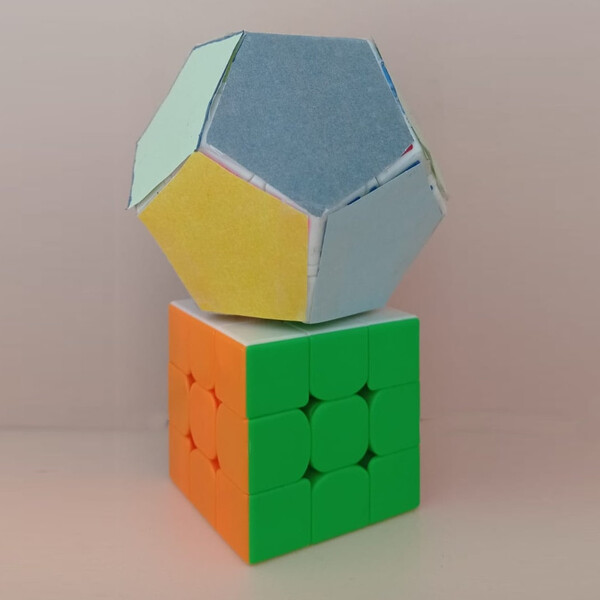
\includegraphics[width=0.36\textwidth]{capture/dodecf0.jpg} &
        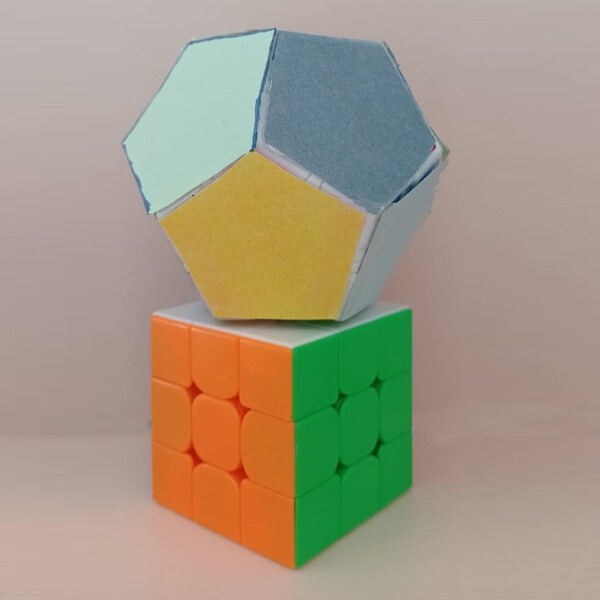
\includegraphics[width=0.36\textwidth]{capture/dodecf1.jpg} \\
        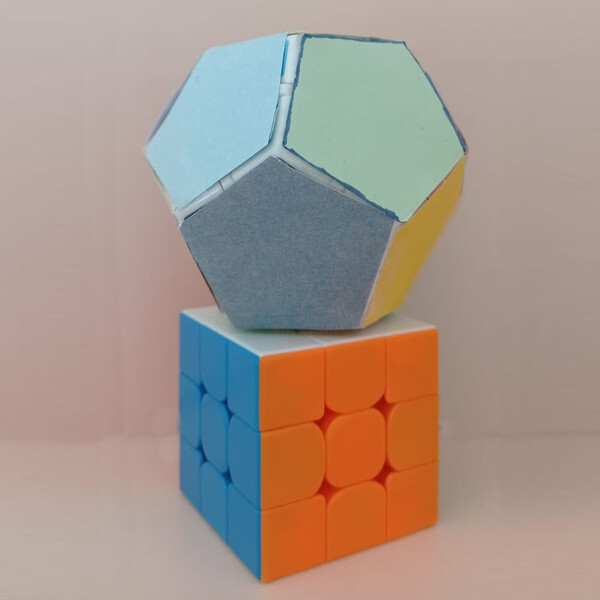
\includegraphics[width=0.36\textwidth]{capture/dodecf2.jpg} &
        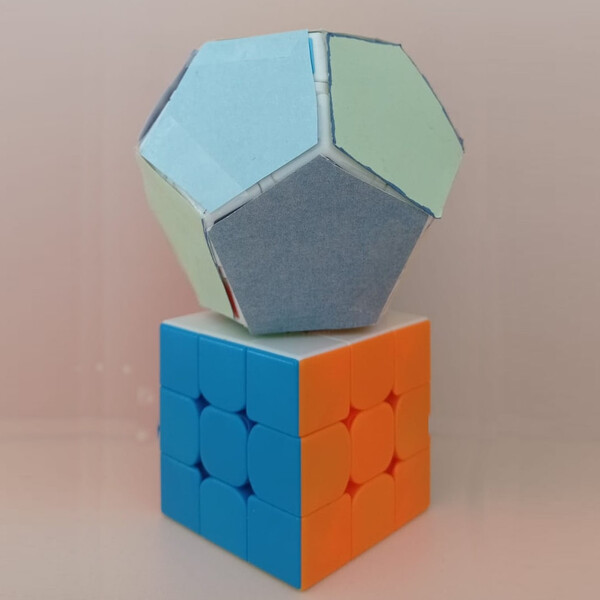
\includegraphics[width=0.36\textwidth]{capture/dodecf3.jpg} \\
        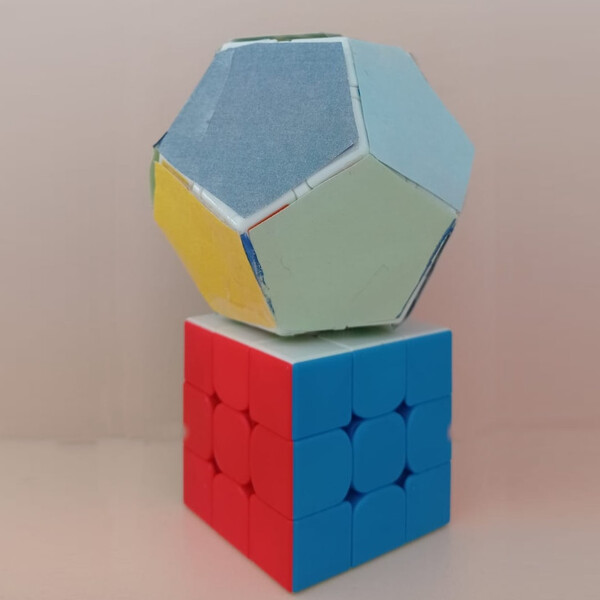
\includegraphics[width=0.36\textwidth]{capture/dodecf4.jpg} &
        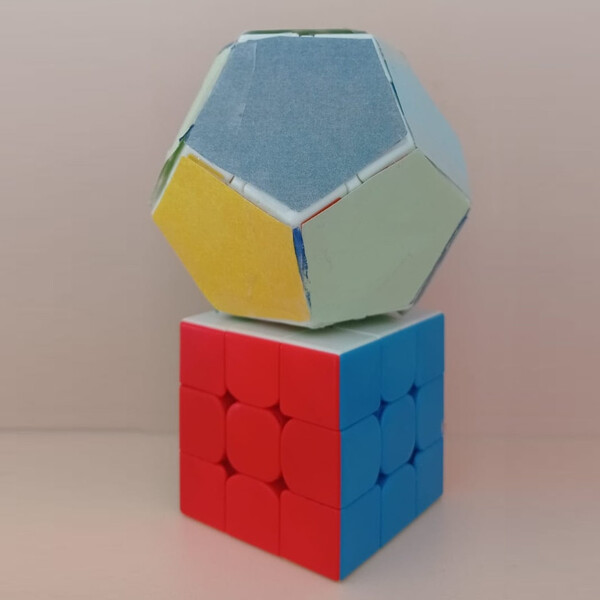
\includegraphics[width=0.36\textwidth]{capture/dodecf5.jpg} \\
        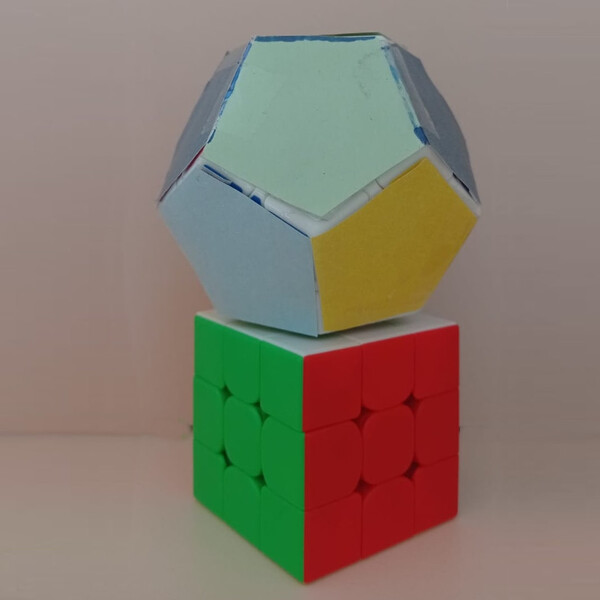
\includegraphics[width=0.36\textwidth]{capture/dodecf6.jpg} &
        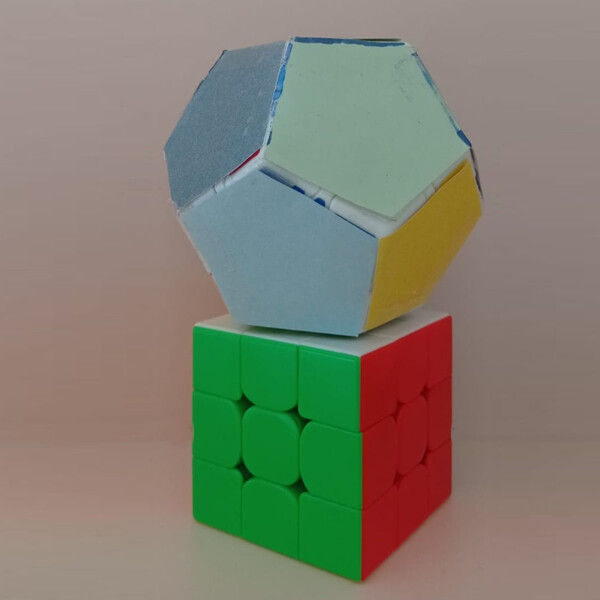
\includegraphics[width=0.36\textwidth]{capture/dodecf7.jpg} \\
    \end{tabular}
\end{minipage}%
\hfill
\begin{minipage}{0.60\textwidth}
    \centering
    \setlength{\tabcolsep}{0pt}
    \renewcommand{\arraystretch}{0}
    \begin{tabular}{c}
        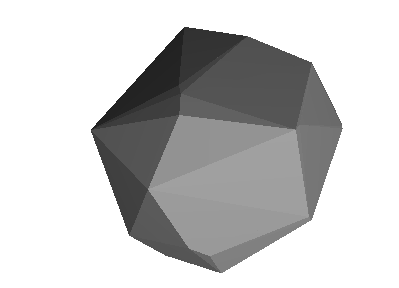
\includegraphics[width=0.72\textwidth]{capture/dodec_vrai.png} \\
    \end{tabular}
    \vspace{0.5em}

    {\tiny \textit{visualisation sur viewstl.com}}
\end{minipage}
\end{frame}


\begin{frame}{La pyramide}
\begin{minipage}{0.40\textwidth}
    \centering
    \setlength{\tabcolsep}{0pt}
    \renewcommand{\arraystretch}{0}
    \begin{tabular}{cc}
        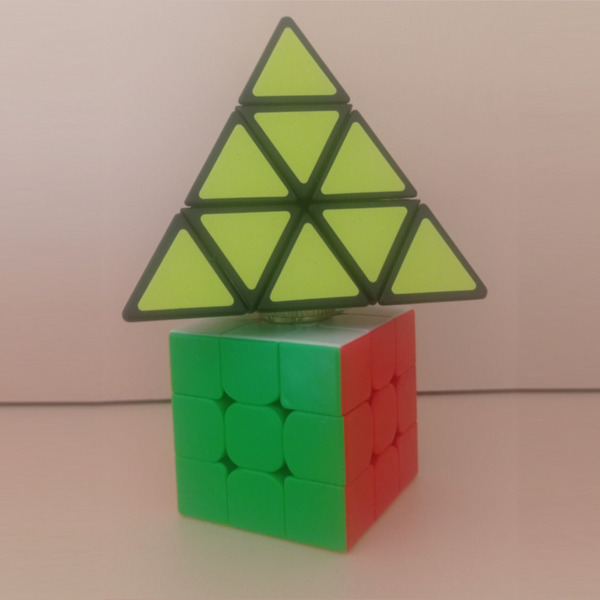
\includegraphics[width=0.36\textwidth]{capture/pyra0.jpg} &
        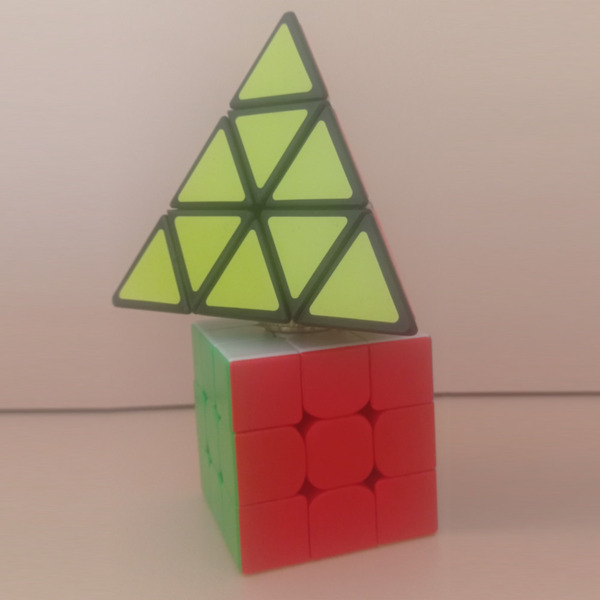
\includegraphics[width=0.36\textwidth]{capture/pyra1.jpg} \\ 
        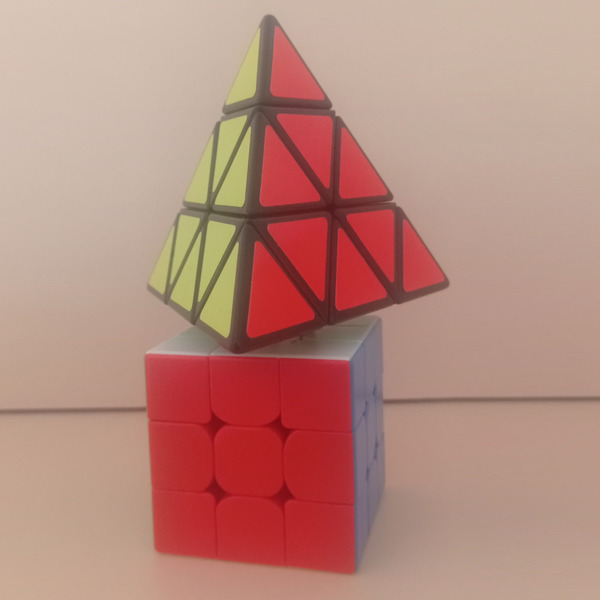
\includegraphics[width=0.36\textwidth]{capture/pyra2.jpg} &
        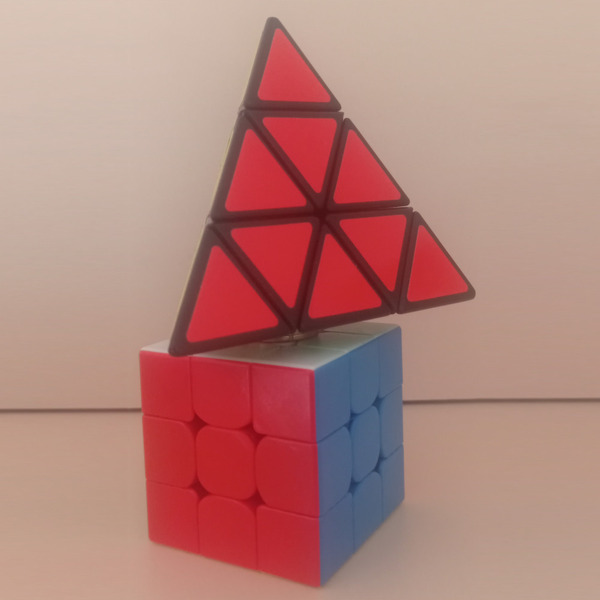
\includegraphics[width=0.36\textwidth]{capture/pyra3.jpg} \\
        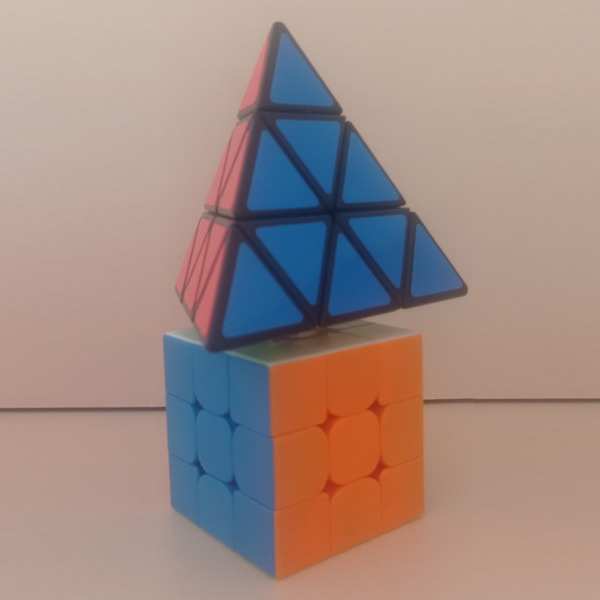
\includegraphics[width=0.36\textwidth]{capture/pyra4.jpg} &
        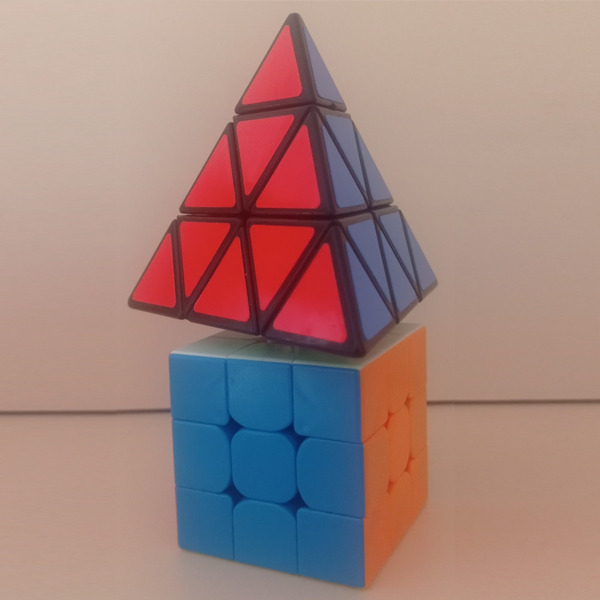
\includegraphics[width=0.36\textwidth]{capture/pyra5.jpg} \\
        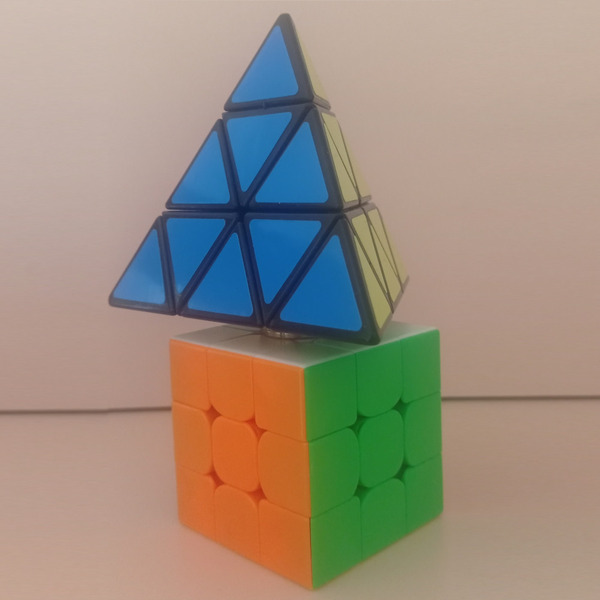
\includegraphics[width=0.36\textwidth]{capture/pyra6.jpg} &
        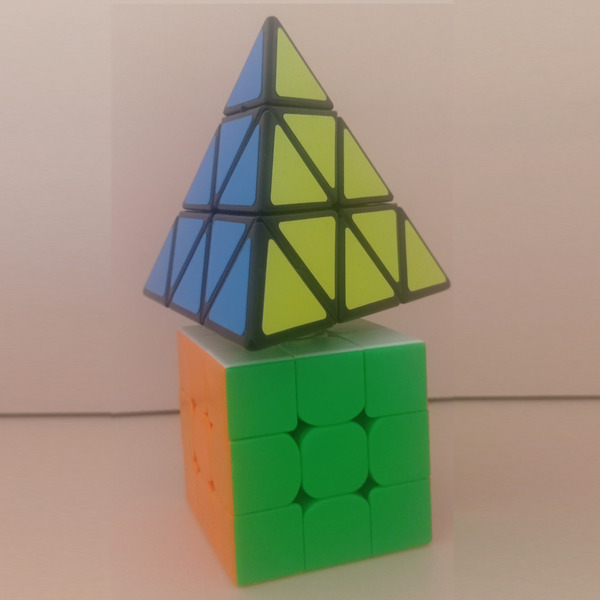
\includegraphics[width=0.36\textwidth]{capture/pyra7.jpg} \\
    \end{tabular}
\end{minipage}%
\hfill
\begin{minipage}{0.60\textwidth}
    \centering
    \setlength{\tabcolsep}{0pt}
    \renewcommand{\arraystretch}{0}
    \begin{tabular}{cc}
        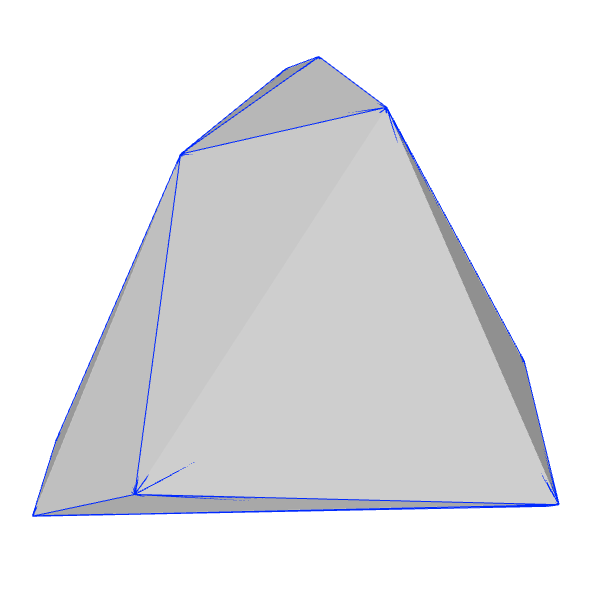
\includegraphics[width=0.40\textwidth]{capture/face1.png} &
        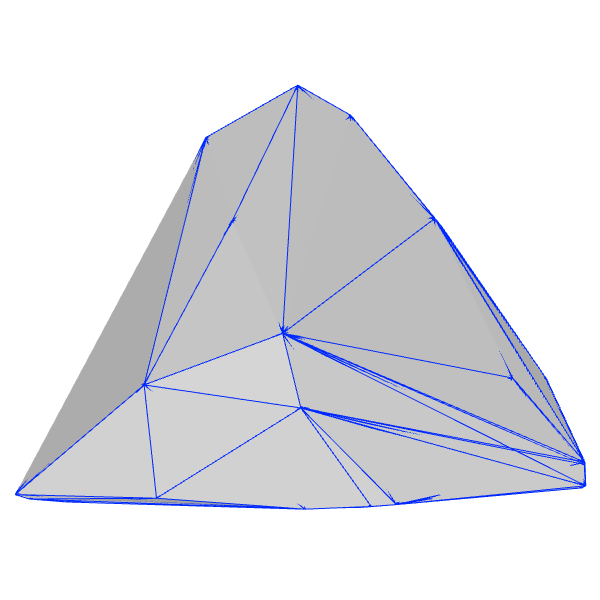
\includegraphics[width=0.40\textwidth]{capture/face2.png} \\
        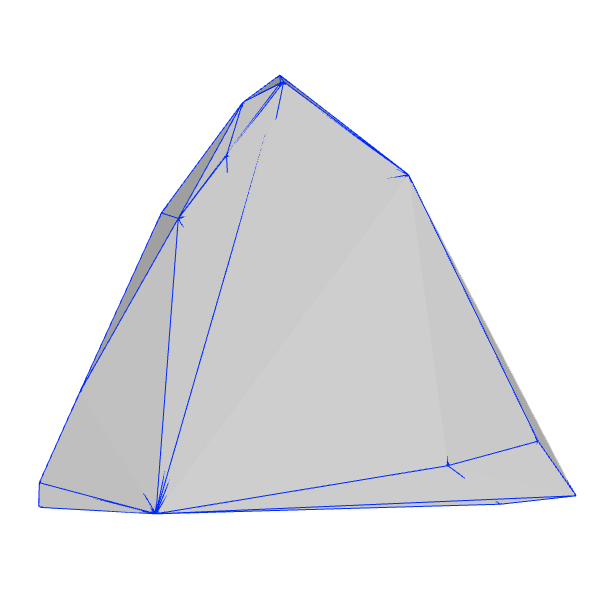
\includegraphics[width=0.40\textwidth]{capture/face3.png} &
        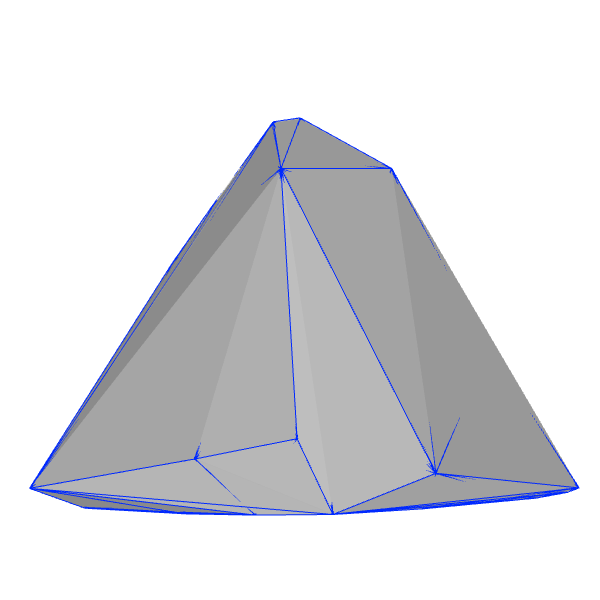
\includegraphics[width=0.40\textwidth]{capture/profil.png} \\
    \end{tabular}
    \vspace{0.2em}

    {\tiny \textit{visualisation sur 3dviewer.net}}
\end{minipage}
\end{frame}

%++++++++++++++++++++++++++++++++++++++++++++++++
\subsection{Des pistes d'amélioration}

%------------------------------------------------

%++++++++++++++++++++++++++++++++++++++++++++++++
\subsection{Limite de la méthode}

%------------------------------------------------
\begin{frame}{Une importante sensibilité aux erreurs}
\centering
\begin{minipage}{0.45\textwidth}
    \centering
    \begin{tikzpicture}
      \node[anchor=south west, inner sep=0] (img1) at (0,0) {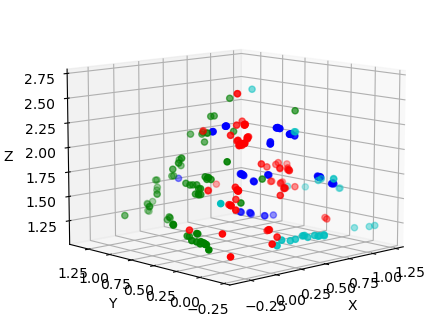
\includegraphics[width=\linewidth]{capture/reconstruit_pyra.png}};
        \begin{scope}[x={(img1.south east)}, y={(img1.north west)}]
            \draw[red, thick] (0.28,0.35) circle [radius=0.03]; % Ajuste les coordonnées
        \end{scope}
    \end{tikzpicture}
    
    \vspace{0.3em}

    \small\textit{points localisés par le programme}
\end{minipage}
\hfill
\begin{minipage}{0.45\textwidth}
    \centering
    \begin{tikzpicture}
      \node[anchor=south west, inner sep=0] (img1) at (0,0) {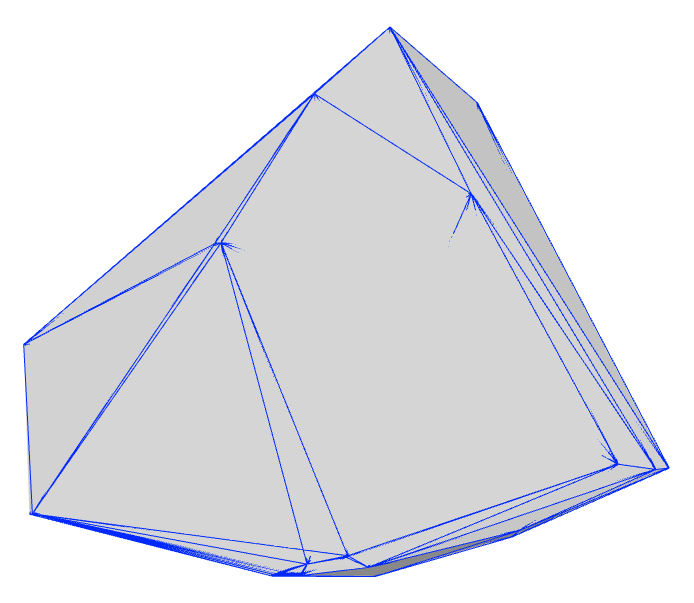
\includegraphics[width=\linewidth]{capture/erreur.png}};
        \begin{scope}[x={(img1.south east)}, y={(img1.north west)}]
            \draw[red, thick] (0.04,0.42) circle [radius=0.03]; % Ajuste les coordonnées
        \end{scope}
    \end{tikzpicture}
    
    \vspace{0.3em}
  \begin{flushleft}
    \small\textit{enveloppe convexe visualisé avec 3dview.net}
  \end{flushleft}

\end{minipage}
\end{frame}

% Slide de test/conclusion
\begin{frame}
  test
\end{frame}

\end{document}
